\documentclass[11pt]{article}

\usepackage[]{acl}

\usepackage{times}
\usepackage{latexsym}
\usepackage[T1]{fontenc}
\usepackage[utf8]{inputenc}
\usepackage{microtype}
\usepackage{inconsolata}
\usepackage{graphicx}
\usepackage{amsmath}
\usepackage{cuted}
\usepackage{caption}

\pagestyle{plain}

\title{Lexical Functions to Improve Lexical Competence}

\author{
    \textbf{Na An\textsuperscript{1}},
    \textbf{Gabriel Beaudoin\textsuperscript{2}},
    \textbf{Noah Tremblay Taillon\textsuperscript{3}}
    \\
    \textsuperscript{1} na.an1@umontreal.ca,
    \textsuperscript{2} gabriel.beaudoin.3@umontreal.ca,\\
    \textsuperscript{3} noah.tremblay.taillon@umontreal.ca
    }

\begin{document}
\maketitle
\thispagestyle{plain}
\begin{abstract}
Large language models exhibit strong performance across many natural language
processing tasks, yet their understanding of fine-grained lexical relations
remains limited compared to that of human native speakers. Recent work has used 
the Meaning-Text Theory (MTT) to evaluate models' lexical competence through
lexical functions, but has focused primarily on evaluation rather than
on model improvement. In this project, we propose a structured dataset of French
lexical units annotated with lexical functions derived from the French Lexical
Network. We used this dataset to fine-tune and evaluate three language models,
assessing whether explicit training on a structured description of natural
language improves models' lexical understanding and their ability to generalize
beyond memorized lexeme pairs. 
Our results show that structural injection tripled Qwen2.5-7B's lexical competence, but effectiveness varied; Mistral-7B experienced catastrophic forgetting and FlauBERT showed minimal change. No general NLU gains were observed on the COLE benchmark.
\end{abstract}

\section{Introduction}
Modern natural language processing systems, particularly Large Language Models (LLMs), achieve strong performance across many natural language tasks. However, their understanding of fine-grained lexical relations specifically the meaning of words and the semantic relations between them remains limited. To address this, we rely on the Meaning-Text Theory (MTT) \cite{melcukVersLinguistiqueSensTexte1997}, which formalizes relations between lexical units using Lexical Functions (LFs). 

While previous research has utilized LFs primarily for evaluating models' lexical competence, our project aims to investigate whether explicit structural injection of these functions can fundamentally improve LLMs' NLU capabilities. We prepared a structured dataset derived from the French Lexical Network (fr-LN) and fine-tuned three selected architectures. We then analyzed the impact of structured lexical knowledge versus standard text exposure. 

In summary, our experiments reveal that while fine-tuned models can achieve a significantly higher understanding of structured lexical relations, notably Qwen2.5-7B which showed a marked improvement on lexical function tasks, these gains are architecture dependent. We observe a trade-off between specialized lexical competence and general stability, as evidenced by the catastrophic forgetting observed in Mistral-7B and the relative stagnation of FlauBERT.

\section{Related Work}\label{sec:relwork}
In order to evaluate language models' natural language understanding (NLU), benchmarks need enough generality to quantify models' linguistic capabilities
\citep{niSurveyLargeLanguage2025}. GLUE \cite{niSurveyLargeLanguage2025}
proposed the first unified benchmark, giving a single score to quantify a
model's performance. Following in the steps of GLUE,
FLUE, a French specific benchmark composed of six linguistic evaluation tasks,
was proposed \citep{leFlauBERTUnsupervisedLanguage2020}. Inspired by this work,
but wanting to add more diversity and subtility to the evaluation, COLE was
created, proposing a 23 tasks evaluation benchmark with a single aggregated
score \citep{beaucheminCOLEComprehensiveBenchmark2025}. 

While general NLU benchmarks are useful, they do not allow for a fine-grained
evaluation of a specific linguistic evaluation, such as lexical capabilities.

The French Lexical Network (fr-LN) \citep{11403/lexical-system-fr/v3.2} is a
formal French lexicon following the MTT, describing a total of $29,976$ lexical
units. LFs are used to describe the relations between all the lexical units,
creating a graph data structure. Using this resource,
\citet{liuAssessingBERTsSensitivity2024} proposed 
an evaluation procedure to assess CamemBERT's \cite{martin-etal-2020-camembert}
understanding of French idioms. \citet{petrovQALFFrenchQuestionAnswering2025}
proposed the Q\&A-LF benchmark to evaluation models' lexical knowledge using
LFs. Using a fixed template prompt design for 15 selected lexical functions,
the authors found that tested language models generally excel when needed to use
morphological evidence, but struggle on tasks involving world conception and
creative reasoning, demonstrating the absence of structured semantic
mapping. Similarly, \citet{liEvaluationCompetenceLexicale2025} used 82 LFs to
compare language models.

These MTT specific evaluation procedures tend to remove rare LFs in their
testing, in order to have a more general score. To our knowledge, no prior work
proposed to enhance models with LFs knowledge explicitly.

\section{Method}
We employed a parameter-efficient fine-tuning approach to verify if explicit structural injection of lexical functions improves linguistic competence. Our primary objective was to compare the performance of fine-tuned models against their base versions to determine if explicit training yields a better understanding of abstract lexical relations.

To achieve this, we relied on Low-Rank Adaptation (LoRA) \citep{LoRA}. LoRA is significantly more cost-effective and computationally efficient than full fine-tuning, allowing us to inject specific Meaning-Text Theory (MTT) constraints without the prohibitive resource costs of updating all model parameters. 

We applied this methodology to three distinct architectures: Mistral-7B \citep{jiangMistral7B2023} for its modern and strong multilingual architecture; Qwen2.5-7B \citep{qwen2} for its instruction-tuned multilingual capabilities; and FlauBERT \citep{leFlauBERTUnsupervisedLanguage2020}, a strong French-specific model. This diversity in models, while maintaining a manageable size for academic experimentation, allowed for a broader understanding of language models' capacities regarding Lexical Functions (LFs).

\section{Experiments}
The code and datasets for this project are available at \url{https://github.com/GabrielBeaudoinUdem/ift6289-project}. The repository is structured to facilitate reproducibility, including clear instructions on environment setup and execution.

\subsection{Datasets}
We created a structured dataset based on the French Lexical Network (fr-LN) \citep{11403/lexical-system-fr/v3.2} formatted in JSON. This structure includes the part of speech (POS), specific senses to handle polysemy, relevant LFs, and an in-context example of the vocable. While all this data is available in fr-LN, our contribution involved structuring it appropriately for model optimization rather than purely for evaluation. Because some LFs have very few instances in fr-LN, we established a minimum occurrence threshold to ensure consistency across the dataset. The dataset was divided into an 80\%/20\% train-test split for our experiments.

\subsection{Baselines}
Our primary baselines were the original, un-finetuned versions of the three selected models (Mistral-7B, Qwen2.5-7B, and FlauBERT). We prompted these original base models to perform the tasks without any weight updates to establish their initial capabilities. 

Additionally, to ensure that any observed performance gains stemmed specifically from the injection of structured lexical knowledge rather than simply from further exposure to the French language, we introduced a secondary fine-tuning baseline. For this, we fine-tuned the base models on a comparable volume of unstructured, raw French text extracted from Wikipedia. Comparing our LF-finetuned models against this Wikipedia-finetuned baseline allowed us to confidently isolate the impact of the structured Meaning-Text Theory annotations versus the mere addition of French linguistic data.

\subsection{Evaluation Methods}
We performed a two-step evaluation procedure. First, we conducted a supervised-learning inspired evaluation on the 20\% test split. Following the evaluation procedure of \citet{petrovQALFFrenchQuestionAnswering2025}, we created fixed query templates for every LF in our dataset. For example, a prompt for the $S_0$ function is \textit{"What noun corresponds to the verb <<Verb>>?"}, asking for a single lexical unit answer. 

We used Exact Match (EM) and Contain Match (CM) \citep{petrovQALFFrenchQuestionAnswering2025} to quantify the models' answers, alongside Accuracy and F1 score. CM is particularly useful to determine if the model's answer contains the desired output, as models often fail to respect the "single lexical unit" constraint. The second evaluation step utilized the COLE benchmark \citep{beaucheminCOLEComprehensiveBenchmark2025} to assess whether learning LFs enables better general natural language understanding beyond specific LF tasks.

\subsection{Experimental Results}
After comparing full fine-tuning and Low-Rank Adaptation (LoRA), we concluded that LoRA was better suited for our task as it allowed us to inject Meaning-Text Theory constraints without the high resource cost of full parameter updates. We implemented our experiments using the HuggingFace transformers and peft libraries. For Mistral-7B-v0.1 and Qwen2.5-7B, we set the LoRA rank to $r=16$ and $\alpha=32$, targeting the query, key, value, and output projections. These models were trained for 1 epoch on local MPS hardware with a $1 \times 10^{-4}$ learning rate and an effective batch size of 16, using a subset of 5,000 examples and their respective instruction templates (\texttt{[INST]} and ChatML). FlauBERT was fine-tuned for 3 epochs on CUDA hardware with a learning rate of $3 \times 10^{-5}$ using an MLM-based template. All models were trained using the AdamW optimizer and gradient checkpointing to manage memory constraints.

\subsection{Results and Analysis}

% \begin{strip}
% \centering
% \resizebox{\textwidth}{!}{
% \begin{tabular}{lccccccccc}
% \hline
% \textbf{Tâche} & \textbf{FlauBERT Base} & \textbf{FlauBERT Wiki} & \textbf{FlauBERT LF} & \textbf{Qwen2.5 Base} & \textbf{Qwen2.5 Wiki} & \textbf{Qwen2.5 LF} & \textbf{Mistral Base} & \textbf{Mistral Wiki} & \textbf{Mistral LF} \\ \hline
% allocine & 54.00\% & 56.00\% & 57.00\% & 70.00\% & 90.00\% & 96.00\% & 82.00\% & 79.00\% & 0.00\% \\
% daccord & 100.00\% & 100.00\% & 100.00\% & 0.00\% & 0.00\% & 0.00\% & 0.00\% & 0.00\% & 0.00\% \\
% fracas & 0.00\% & 0.00\% & 0.00\% & 62.00\% & 44.00\% & 63.00\% & 54.00\% & 52.00\% & 0.00\% \\
% french\_boolq & 100.00\% & 100.00\% & 100.00\% & 0.00\% & 0.00\% & 0.00\% & 0.00\% & 0.00\% & 0.00\% \\
% gqnli & 44.44\% & 44.44\% & 55.56\% & 40.74\% & 33.33\% & 37.04\% & 22.22\% & 33.33\% & 0.00\% \\
% lingnli & 100.00\% & 100.00\% & 100.00\% & 47.00\% & 11.00\% & 60.00\% & 75.00\% & 61.00\% & 0.00\% \\
% mms & 100.00\% & 100.00\% & 100.00\% & 0.00\% & 0.00\% & 0.00\% & 0.00\% & 0.00\% & 0.00\% \\
% mnli-nineeleven-fr-mt & 100.00\% & 100.00\% & 100.00\% & 0.00\% & 0.00\% & 0.00\% & 0.00\% & 0.00\% & 0.00\% \\
% multiblimp & 53.00\% & 53.00\% & 53.00\% & 89.00\% & 90.00\% & 84.00\% & 65.00\% & 63.00\% & 21.00\% \\
% paws\_x & 45.00\% & 45.00\% & 45.00\% & 73.00\% & 39.00\% & 69.00\% & 45.00\% & 32.00\% & 1.00\% \\
% qfrblimp & 59.00\% & 59.00\% & 59.00\% & 81.00\% & 78.00\% & 77.00\% & 60.00\% & 61.00\% & 41.00\% \\
% qfrcola & 70.00\% & 70.00\% & 69.00\% & 78.00\% & 61.00\% & 77.00\% & 72.00\% & 71.00\% & 0.00\% \\
% rte3-french & 25.00\% & 27.00\% & 32.00\% & 61.00\% & 23.00\% & 53.00\% & 37.00\% & 43.00\% & 0.00\% \\
% sickfr & 18.00\% & 18.00\% & 15.00\% & 69.00\% & 66.00\% & 62.00\% & 27.00\% & 25.00\% & 0.00\% \\
% sts22 & 19.00\% & 19.00\% & 21.00\% & 14.00\% & 25.00\% & 23.00\% & 13.00\% & 12.00\% & 0.00\% \\
% wino\_x\_lm & 100.00\% & 100.00\% & 100.00\% & 0.00\% & 0.00\% & 0.00\% & 0.00\% & 0.00\% & 0.00\% \\
% wino\_x\_mt & 100.00\% & 100.00\% & 100.00\% & 0.00\% & 0.00\% & 0.00\% & 0.00\% & 0.00\% & 0.00\% \\
% xnli & 33.00\% & 35.00\% & 31.00\% & 70.00\% & 75.00\% & 62.00\% & 47.00\% & 43.00\% & 0.00\% \\
% \hline
% \textbf{SCORE COLE (TOTAL)} & \textbf{62.25\%} & \textbf{62.58\%} & \textbf{63.20\%} & \textbf{41.93\%} & \textbf{35.30\%} & \textbf{42.39\%} & \textbf{33.29\%} & \textbf{31.96\%} & \textbf{3.50\%} \\
% \hline
% \end{tabular}
% }
% \captionof{table}{COLE benchmark results}
% \end{strip}

\begin{strip}
\centering
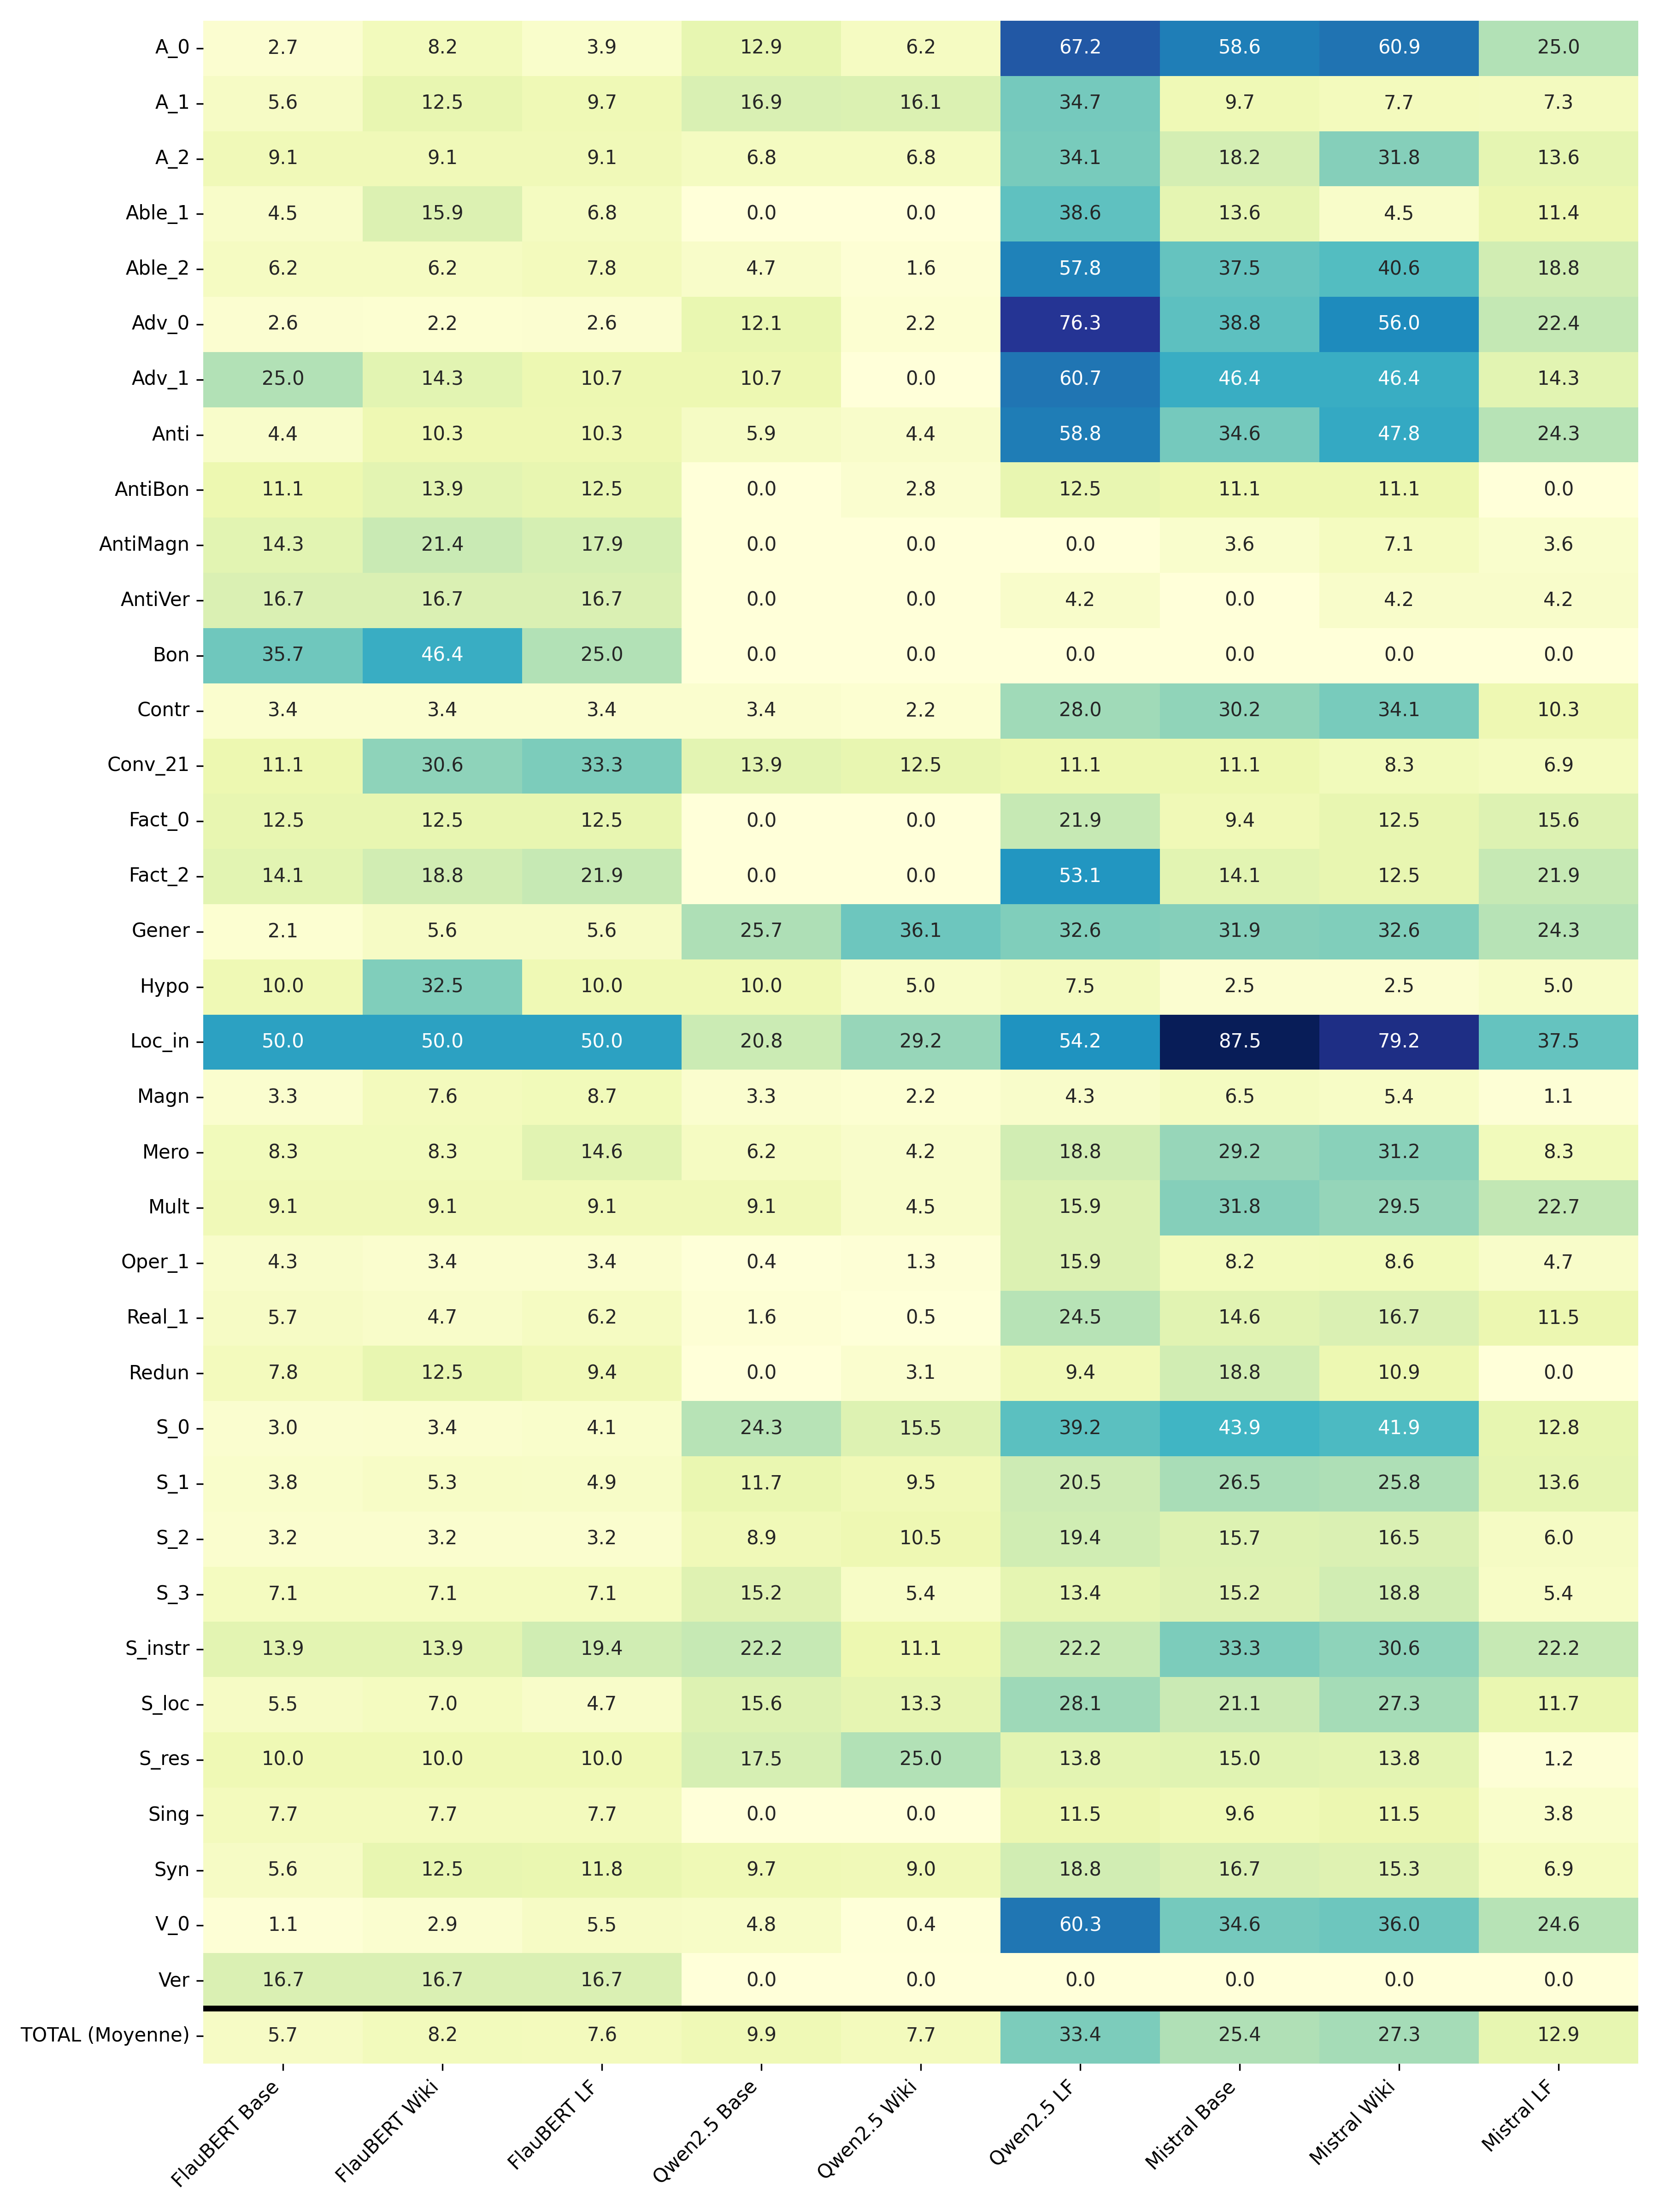
\includegraphics[width=0.9\textwidth]{figures/fl_heatmap.png}
\captionof{figure}{Lexical Functions (LF) benchmark performance heatmap (percentage)}
\label{fig:fl_heatmap}
\end{strip}

The evaluation on the Lexical Functions (LF) benchmark (see Figure \ref{fig:fl_heatmap}) reveals stark differences in how different architectures react to structural knowledge injection. 

Qwen2.5-7B demonstrated the most significant benefit from LF fine-tuning, with its global score jumping from 9.9\% (Base) to 33.4\% (LF). The fine-tuned model performed exceptionally well on functions requiring a change in Part-of-Speech (POS), such as \textit{S\_0}, \textit{V\_0}, and \textit{Adv\_0}. However, rather than acquiring strictly new linguistic knowledge, we hypothesize that the LoRA fine-tuning primarily taught Qwen2.5 how to correctly format its answers to align with the rigid, single-lexeme task constraints, unlocking its pre-existing French capabilities.

Conversely, Mistral-7B experienced a severe performance drop following LF fine-tuning, falling from a robust 25.4\% (Base) to 12.9\% (LF). This indicates catastrophic forgetting and severe overfitting to the training distribution. Interestingly, Mistral Base and Mistral Wiki were surprisingly competitive with the fine-tuned Qwen model, heavily boosted by exceptionally high scores on specific functions like \textit{Loc\_in}, which warrants cautious interpretation of global averages.

FlauBERT exhibited high stability across all configurations, with scores remaining largely similar (ranging from 5.7\% to 8.2\%). We suspect the learning rate may have been too low to induce meaningful parametric shifts for this architecture, leading to a ceiling effect. Notably, FlauBERT Wiki achieved the highest score among the encoder variations. Its slight superiority on the \textit{Hypo} (hyponym) function aligns with the encyclopedic nature of Wikipedia, which is heavily structured around hypernym/hyponym relationships. Curiously, this trend did not extend to the \textit{Gener} function.

Finally, certain categories such as \textit{Ver}, \textit{AntiVer}, \textit{AntiMagn}, and \textit{Bon} proved universally difficult across all models and configurations. This suggests a broader issue of either severe data scarcity in the pre-training corpora for these specific semantic relations, or an inherent difficulty in the tasks themselves. Furthermore, the baseline comparison reveals that fine-tuning on unstructured Wikipedia data does not consistently beat the base models, confirming that simply increasing a model's exposure to French text does not equate to an improved understanding of fine-grained lexical competence.

% \begin{strip}
% \centering
% \resizebox{\textwidth}{!}{
% \begin{tabular}{lccccccccc}
% \hline
% \textbf{Fonction Lexicale} & \textbf{FlauBERT Base} & \textbf{FlauBERT Wiki} & \textbf{FlauBERT LF} & \textbf{Qwen2.5 Base} & \textbf{Qwen2.5 Wiki} & \textbf{Qwen2.5 LF} & \textbf{Mistral Base} & \textbf{Mistral Wiki} & \textbf{Mistral LF} \\ \hline
% A\_0 & 2.7\% & 8.2\% & 3.9\% & 12.9\% & 6.2\% & 67.2\% & 58.6\% & 60.9\% & 25.0\% \\
% A\_1 & 5.6\% & 12.5\% & 9.7\% & 16.9\% & 16.1\% & 34.7\% & 9.7\% & 7.7\% & 7.3\% \\
% A\_2 & 9.1\% & 9.1\% & 9.1\% & 6.8\% & 6.8\% & 34.1\% & 18.2\% & 31.8\% & 13.6\% \\
% Able\_1 & 4.5\% & 15.9\% & 6.8\% & 0.0\% & 0.0\% & 38.6\% & 13.6\% & 4.5\% & 11.4\% \\
% Able\_2 & 6.2\% & 6.2\% & 7.8\% & 4.7\% & 1.6\% & 57.8\% & 37.5\% & 40.6\% & 18.8\% \\
% Adv\_0 & 2.6\% & 2.2\% & 2.6\% & 12.1\% & 2.2\% & 76.3\% & 38.8\% & 56.0\% & 22.4\% \\
% Adv\_1 & 25.0\% & 14.3\% & 10.7\% & 10.7\% & 0.0\% & 60.7\% & 46.4\% & 46.4\% & 14.3\% \\
% Anti & 4.4\% & 10.3\% & 10.3\% & 5.9\% & 4.4\% & 58.8\% & 34.6\% & 47.8\% & 24.3\% \\
% AntiBon & 11.1\% & 13.9\% & 12.5\% & 0.0\% & 2.8\% & 12.5\% & 11.1\% & 11.1\% & 0.0\% \\
% AntiMagn & 14.3\% & 21.4\% & 17.9\% & 0.0\% & 0.0\% & 0.0\% & 3.6\% & 7.1\% & 3.6\% \\
% AntiVer & 16.7\% & 16.7\% & 16.7\% & 0.0\% & 0.0\% & 4.2\% & 0.0\% & 4.2\% & 4.2\% \\
% Bon & 35.7\% & 46.4\% & 25.0\% & 0.0\% & 0.0\% & 0.0\% & 0.0\% & 0.0\% & 0.0\% \\
% Contr & 3.4\% & 3.4\% & 3.4\% & 3.4\% & 2.2\% & 28.0\% & 30.2\% & 34.1\% & 10.3\% \\
% Conv\_21 & 11.1\% & 30.6\% & 33.3\% & 13.9\% & 12.5\% & 11.1\% & 11.1\% & 8.3\% & 6.9\% \\
% Fact\_0 & 12.5\% & 12.5\% & 12.5\% & 0.0\% & 0.0\% & 21.9\% & 9.4\% & 12.5\% & 15.6\% \\
% Fact\_2 & 14.1\% & 18.8\% & 21.9\% & 0.0\% & 0.0\% & 53.1\% & 14.1\% & 12.5\% & 21.9\% \\
% Gener & 2.1\% & 5.6\% & 5.6\% & 25.7\% & 36.1\% & 32.6\% & 31.9\% & 32.6\% & 24.3\% \\
% Hypo & 10.0\% & 32.5\% & 10.0\% & 10.0\% & 5.0\% & 7.5\% & 2.5\% & 2.5\% & 5.0\% \\
% Loc\_in & 50.0\% & 50.0\% & 50.0\% & 20.8\% & 29.2\% & 54.2\% & 87.5\% & 79.2\% & 37.5\% \\
% Magn & 3.3\% & 7.6\% & 8.7\% & 3.3\% & 2.2\% & 4.3\% & 6.5\% & 5.4\% & 1.1\% \\
% Mero & 8.3\% & 8.3\% & 14.6\% & 6.2\% & 4.2\% & 18.8\% & 29.2\% & 31.2\% & 8.3\% \\
% Mult & 9.1\% & 9.1\% & 9.1\% & 9.1\% & 4.5\% & 15.9\% & 31.8\% & 29.5\% & 22.7\% \\
% Oper\_1 & 4.3\% & 3.4\% & 3.4\% & 0.4\% & 1.3\% & 15.9\% & 8.2\% & 8.6\% & 4.7\% \\
% Real\_1 & 5.7\% & 4.7\% & 6.2\% & 1.6\% & 0.5\% & 24.5\% & 14.6\% & 16.7\% & 11.5\% \\
% Redun & 7.8\% & 12.5\% & 9.4\% & 0.0\% & 3.1\% & 9.4\% & 18.8\% & 10.9\% & 0.0\% \\
% S\_0 & 3.0\% & 3.4\% & 4.1\% & 24.3\% & 15.5\% & 39.2\% & 43.9\% & 41.9\% & 12.8\% \\
% S\_1 & 3.8\% & 5.3\% & 4.9\% & 11.7\% & 9.5\% & 20.5\% & 26.5\% & 25.8\% & 13.6\% \\
% S\_2 & 3.2\% & 3.2\% & 3.2\% & 8.9\% & 10.5\% & 19.4\% & 15.7\% & 16.5\% & 6.0\% \\
% S\_3 & 7.1\% & 7.1\% & 7.1\% & 15.2\% & 5.4\% & 13.4\% & 15.2\% & 18.8\% & 5.4\% \\
% S\_instr & 13.9\% & 13.9\% & 19.4\% & 22.2\% & 11.1\% & 22.2\% & 33.3\% & 30.6\% & 22.2\% \\
% S\_loc & 5.5\% & 7.0\% & 4.7\% & 15.6\% & 13.3\% & 28.1\% & 21.1\% & 27.3\% & 11.7\% \\
% S\_res & 10.0\% & 10.0\% & 10.0\% & 17.5\% & 25.0\% & 13.8\% & 15.0\% & 13.8\% & 1.2\% \\
% Sing & 7.7\% & 7.7\% & 7.7\% & 0.0\% & 0.0\% & 11.5\% & 9.6\% & 11.5\% & 3.8\% \\
% Syn & 5.6\% & 12.5\% & 11.8\% & 9.7\% & 9.0\% & 18.8\% & 16.7\% & 15.3\% & 6.9\% \\
% V\_0 & 1.1\% & 2.9\% & 5.5\% & 4.8\% & 0.4\% & 60.3\% & 34.6\% & 36.0\% & 24.6\% \\
% Ver & 16.7\% & 16.7\% & 16.7\% & 0.0\% & 0.0\% & 0.0\% & 0.0\% & 0.0\% & 0.0\% \\
% \hline
% \textbf{TOTAL (Moyenne)} & \textbf{5.7\%} & \textbf{8.2\%} & \textbf{7.6\%} & \textbf{9.9\%} & \textbf{7.7\%} & \textbf{33.4\%} & \textbf{25.4\%} & \textbf{27.3\%} & \textbf{12.9\%} \\
% \hline
% \end{tabular}
% }
% \captionof{table}{Lexical Functions (LF) benchmark results}
% \end{strip}



\begin{figure*}[t]
\centering
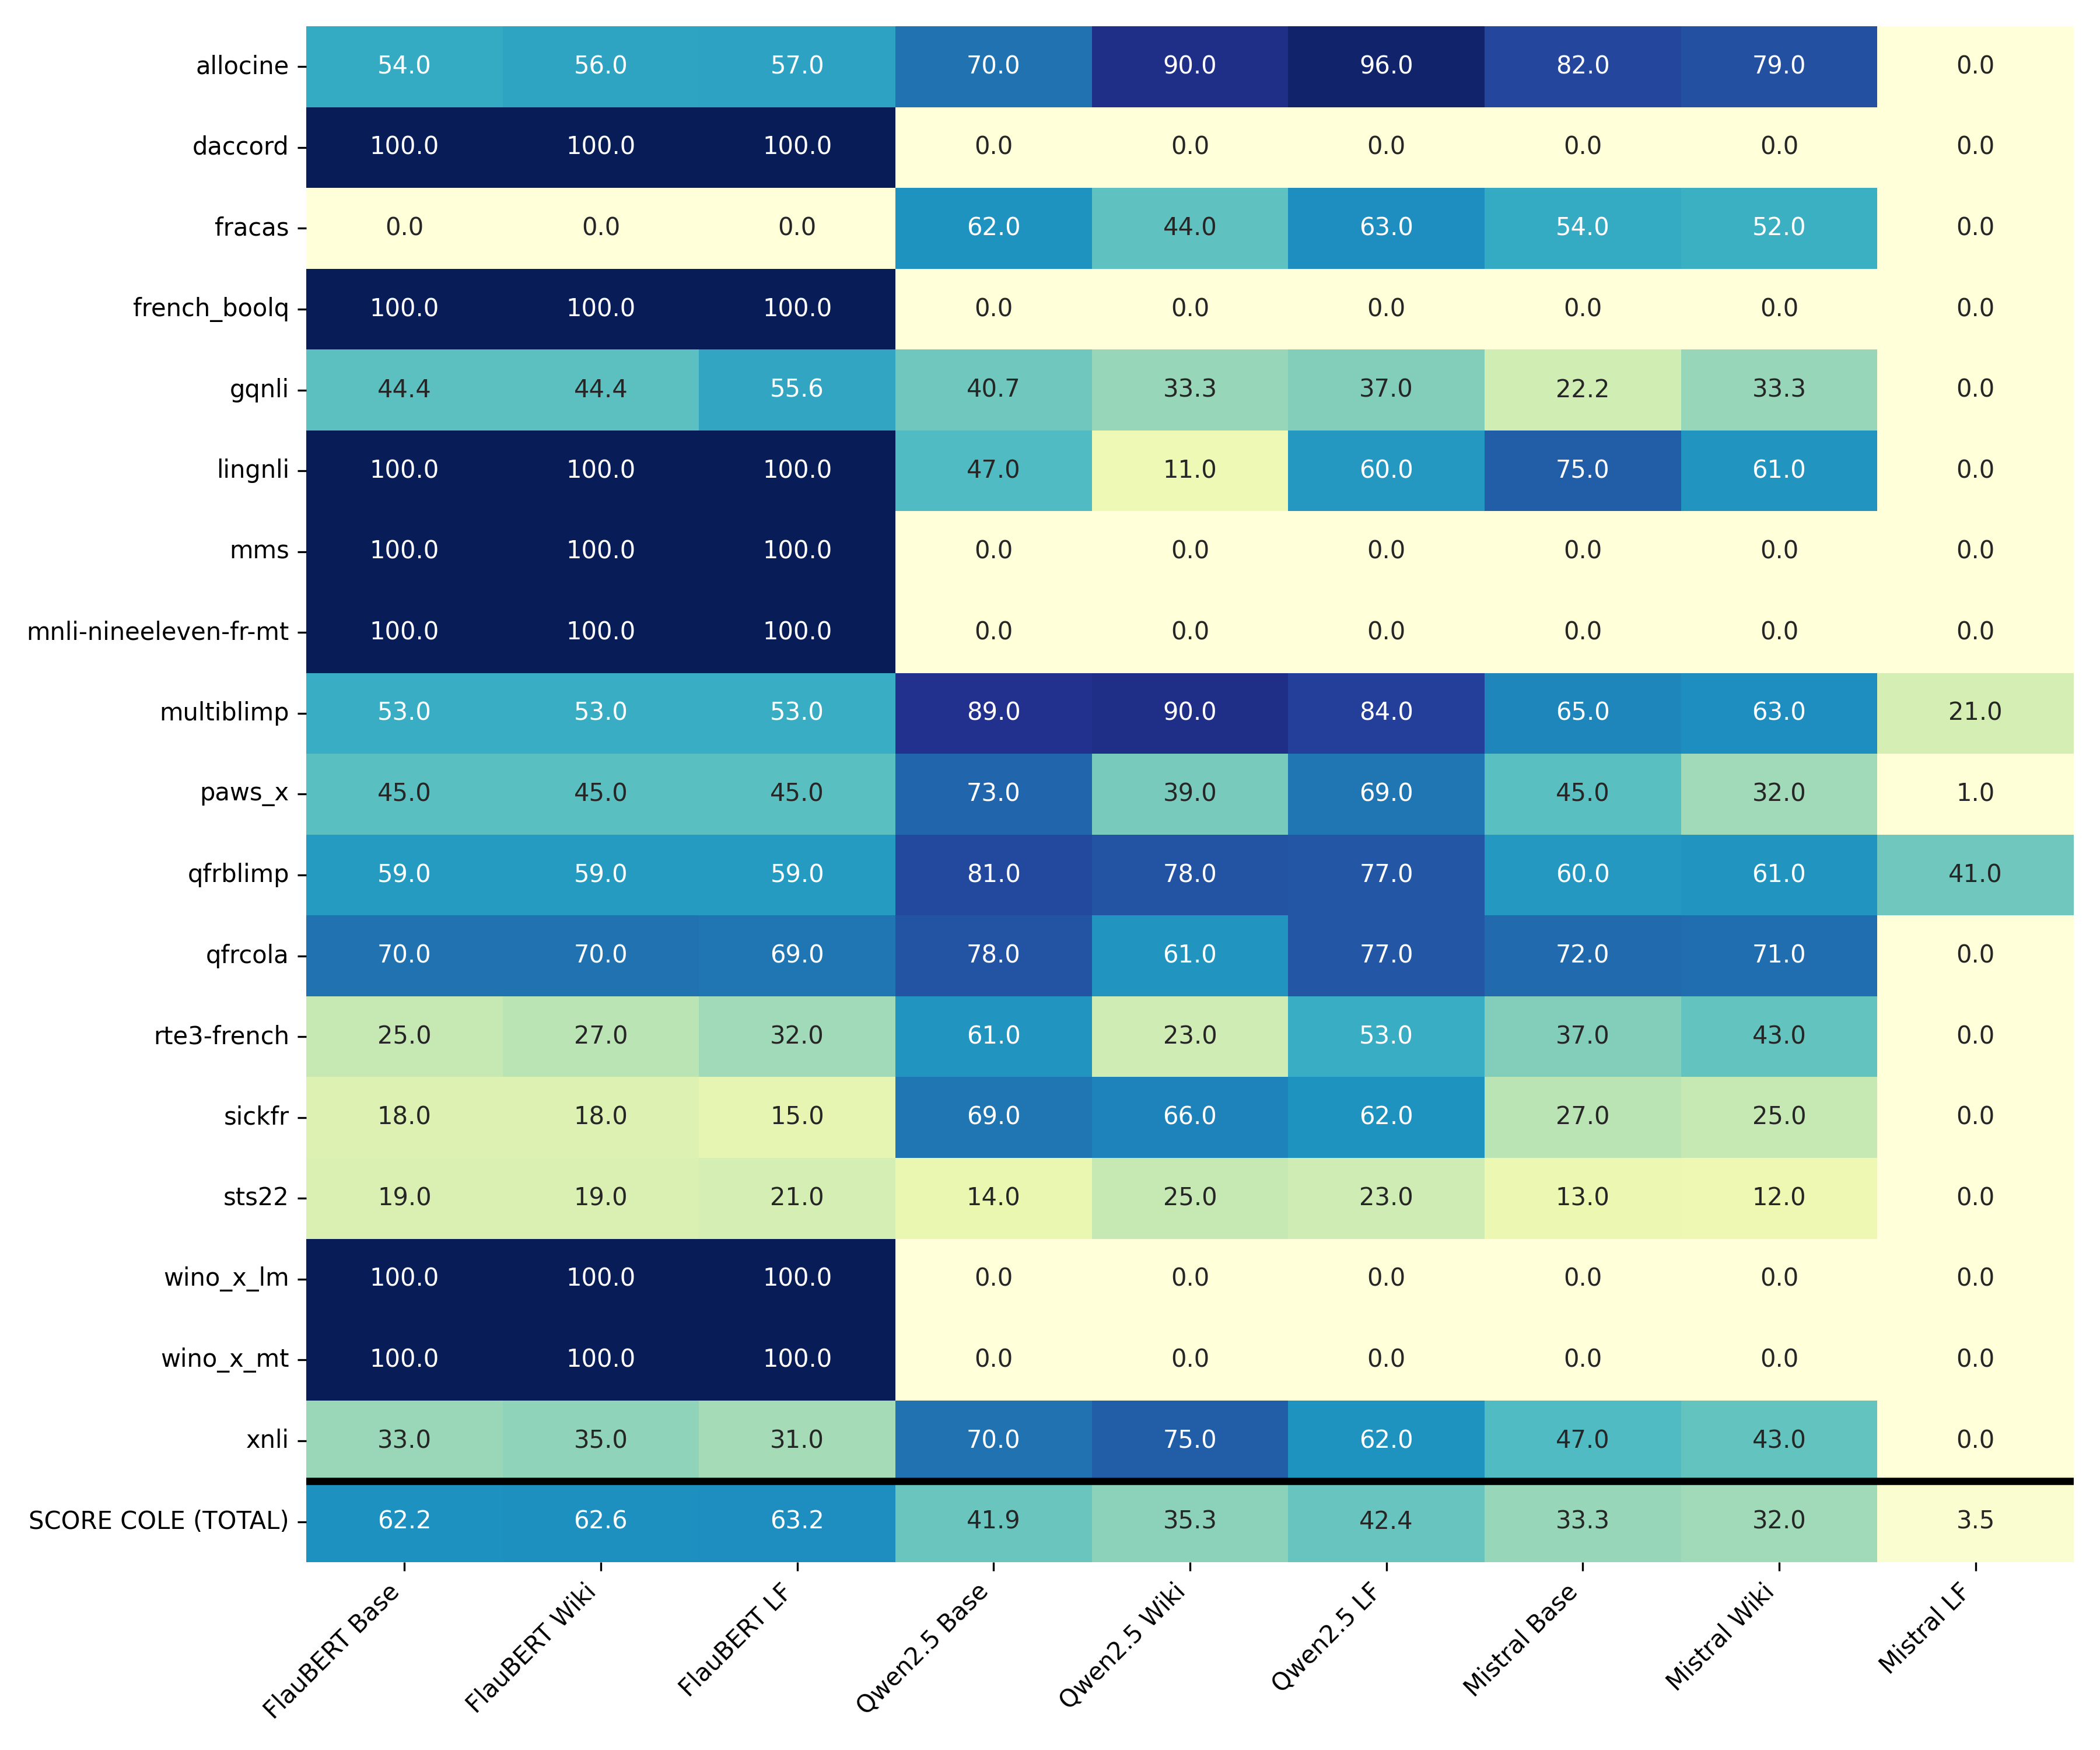
\includegraphics[width=0.9\textwidth]{figures/cole_heatmap.png}
\captionof{figure}{COLE benchmark performance heatmap (percentage)}
\label{fig:cole_heatmap}
\end{figure*}

To evaluate whether explicit lexical training translates to broader natural language understanding, we tested the models on the COLE benchmark (see Figure \ref{fig:cole_heatmap}). The most striking observation is the absolute divergence between the encoder (FlauBERT) and the generative decoder architectures (Qwen2.5, Mistral).

FlauBERT achieved near-perfect scores (100\%) on specific classification tasks such as \textit{daccord}, \textit{french\_boolq}, \textit{mms}, and \textit{wino\_x}, while Qwen and Mistral scored exactly 0.0\% on these same metrics. This massive disparity strongly suggests an evaluation methodology artifact rather than a true capability deficit. COLE tasks are highly optimized for encoder models that output specific classification labels. Generative LLMs, without specialized few-shot prompting, struggle to output the exact expected token, leading to artificial 0.0\% scores. Consequently, COLE scores for the generative models are likely severe underestimates of their actual NLU capabilities.

Despite these formatting hurdles, Qwen2.5 LF showed a minor global score increase compared to its base version, driven by gains in tasks like \textit{allocine} (sentiment analysis). FlauBERT remained mostly stable, though FlauBERT LF exhibited an unexpected improvement on the \textit{gqnli} natural language inference task (categorizing contradictions vs. neutral statements).

However, Mistral-7B's performance on COLE confirms the catastrophic forgetting observed in the LF benchmark. The Mistral LF model's global score collapsed to 3.50\%, scoring 0.0\% on almost all tasks, proving that the model overlearned the specific structure of the LF dataset at the expense of its general language modeling capabilities.

Ultimately, these results highlight a fundamental format mismatch: the COLE benchmark favors encoder models built for classification, while the LF query benchmark favors generative models built to produce specific words. Neither benchmark alone captures the full picture, but our results indicate that while targeted LoRA fine-tuning can teach a generative model to excel at structural semantic mapping (as seen with Qwen), it does not easily generalize to broader NLU tasks and carries a high risk of catastrophic forgetting (as seen with Mistral).

\section{Conclusion}
In this project, we investigated whether explicitly training language models on structured lexical functions, derived from the Meaning-Text Theory, could improve both their specific lexical competence and their general Natural Language Understanding (NLU). To do so, we generated a specialized LF dataset from the French Lexical Network and applied LoRA fine-tuning across three distinct architectures.

Our findings are mixed and highlight the complexity of augmenting LLMs with highly structured linguistic data. On one hand, we observed a resounding success with Qwen2.5, which more than tripled its performance on the Lexical Functions benchmark, proving that structural injection can indeed work when the model architecture and instruction-tuning align well with the training methodology.

On the other hand, we must remain highly cautious regarding the generalizability of these results. Enhancing specific lexical knowledge did not translate into a broader improvement on the general NLU benchmark (COLE). Furthermore, the complete performance collapse observed in the Mistral model serves as a stark reminder of the risks of catastrophic forgetting and formatting-overfit when applying parameter-efficient fine-tuning on highly specific datasets. 

Future work should explore alternative integration methods that are less prone to catastrophic forgetting. Soft-prompting, adapting the LoRA hyperparameters dynamically, or integrating LF data directly during the pre-training or standard alignment phases (RLHF/DPO) might yield a better balance between specialized structural lexical knowledge and robust general linguistic capabilities.

\bibliography{proposal}

\newpage
\appendix
\section{Contributions of Each Team Member}
\begin{itemize}
    \item \textbf{Noah Tremblay Taillon:} Responsible for extracting, cleaning, and preparing the linguistic functions dataset. He also developed the evaluation pipeline and prepared the benchmarking infrastructure for the linguistic functions. Together with Gabriel Beaudoin, he contributed to the writing of the project proposal, the mid-progress report, the final report, and the poster.
    \item \textbf{Gabriel Beaudoin:} Responsible for preparing the Wikipedia baseline dataset and integrating the COLE benchmark. He also led the fine-tuning process and executed the evaluation scripts for the Mistral-7B and Qwen2.5-7B models. Together with Noah Tremblay Taillon, he contributed to the writing of the project proposal, the mid-progress report, the final report, and the poster.
    \item \textbf{Na An:} Responsible for the configuration and fine-tuning of the FlauBERT model, and conducted the performance evaluations for this architecture.
\end{itemize}

\end{document}